\section{Effet Venturi}


On considère un fluide incompressible bafait et en écoulement. L'aire de la section droite est variable. \( A\) et \(B\) sont deux points d'une même ligne de courrant tel que \(z_{A} = z_{B}\). Le débit volumique \(D_{v}\) étant constant, on a :\(s_{A} \cdot v_{A} = s_{B} \cdot v_{B}\).\\
Comme \(s_{A}>s_{B}\), alors \(v_{B}>v_{A}\). La relation de bernoulli appliquée entre \(A\) et \(B\) donne : \\
\[
    P_{A} +\frac{1}{2}\rho v_{A}^{2} = P_{B} +\frac{1}{2}\rho v_{B}^{2} \iff P_{B} = P_{A} + \frac{1}{2}\rho (v_{A}^{2} - v_{B}^{2})<P_{A}
\]
En conclusion, en \(B\) , la vitesse augmente et la pression diminue.
\begin{figure}[!htb]
    \centering
    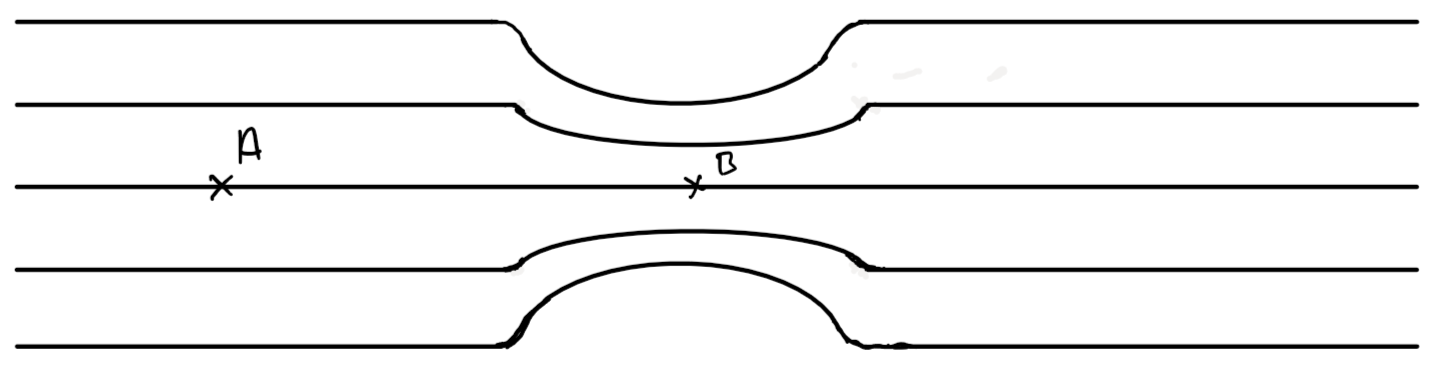
\includegraphics[width=0.8\textwidth]{SchemaVen.png}
    \caption{L'effet Venturi.}
    \label{fig:SchemaVen}
\end{figure}
